\chapter{DESARROLLO DEL EXPERIMENTO}
\section{Determinación y evaluación de alternativas de solución}

En primer lugar, se observó que la empresa cuenta con un amplio portafolio de productos, con más de 20 familias diferentes. Sin embargo, no todas estas familias tienen la misma relevancia en términos de ventas. Para abordar el desafío de predecir las ventas en este diverso conjunto de familias de productos, se llevó a cabo un proceso de selección cuidadoso. Se identificaron y seleccionaron las familias con mayor relevancia en las ventas, basándose en datos históricos y análisis de rendimiento comercial.

\begin{figure}[H]
	\begin{center}
		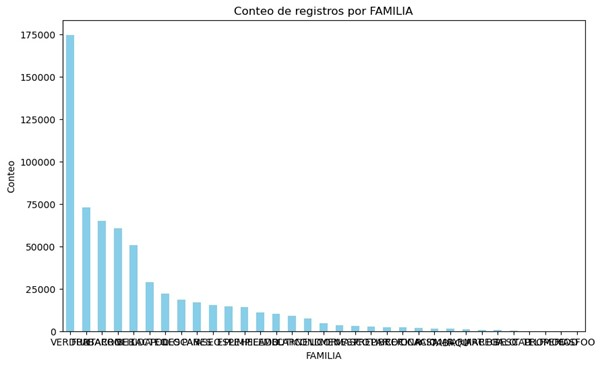
\includegraphics[width=0.9\textwidth]{2/figures/resul1_paper.jpg}
		\caption{Familia de productos}
		\textit{Fuente: Elaboración propia}
		\label{fig11}
	\end{center}
	
\end{figure}

Las familias de productos seleccionadas para el análisis representan una parte significativa de las operaciones comerciales de la empresa.  Se priorizaron  según  su  contribución  a los  ingresos  totales  y  su  impacto  en  la  rentabilidad  general.  Esta selección se basó en datos concretos, incluidos registros de ventas, análisis de tendencias del mercado y consultas con los departamentos de ventas y marketing. Con las familias de productos relevantes identificadas, se procedió a  explorar  diferentes  enfoques  para  predecir  las  ventas  futuras.  Se reconocieron dos alternativas principales, diseñadas para maximizar la utilidad de los datos disponibles y adaptarse a las necesidades específicas de cada familia de productos:



\begin{enumerate}
	\item Utilizar un Único Modelo de Predicción para las Familias Relevantes: En esta alternativa, se propone emplear un único modelo de predicción que abarque todas las familias de productos consideradas relevantes para las ventas. Este modelo se entrenaría utilizando datos históricos recopilados de estas familias y se utilizaría para realizar predicciones en tiempo real. Se considera que esta opción puede simplificar el proceso de predicción y ser más eficiente en términos de recursos y tiempo de implementación. No obstante, existe la preocupación de que este enfoque pueda subutilizar la información específica de cada familia, lo que podría resultar en predicciones menos precisas y adaptadas a las particularidades de cada una.
	
	\item Probar múltiples modelos para cada familia relevante: Esta alternativa implica la evaluación de varios modelos de predicción para cada familia de productos relevante en las ventas. Dado que la empresa cuenta con un amplio conjunto de familias de productos, se seleccionaron las seis más relevantes en términos de ventas. Se considera probar modelos como regresión logística, LSTM y XGBoost, entre otros, para determinar cuál proporciona las mejores métricas de rendimiento para cada familia. Aunque esta opción puede ser más compleja y requerir más recursos computacionales y tiempo de implementación, ofrece la ventaja de una mayor personalización y optimización para cada familia, lo que podría resultar en predicciones más precisas y adaptadas a sus características específicas.
\end{enumerate}



%\begin{table}
%	\centering
%	\begin{tabular}{l|r}
%		Item & Quantity \\\hline
%		Widgets & 42 \\
%		Gadgets & 13
%	\end{tabular}
%	\caption{\label{tab:widgets1}An example table.}
%\end{table}

\section{Propuesta solución}

Esta propuesta, como se explicó anteriormente, implica un enfoque más granular y específico para cada familia de productos seleccionada. En lugar de aplicar un único modelo de predicción a todas las familias, se explorará la idoneidad de múltiples modelos para cada una, teniendo en cuenta sus características individuales y su historial de ventas. Entre estos modelos se encuentran los siguientes:

\begin{itemize}
	\item \textbf{Linear Regression: } Un modelo de regresión lineal que busca la mejor relación lineal entre las variables independientes y la variable dependiente.
	\item \textbf{Decision Tree: } Un modelo basado en árboles de decisión que segmenta los datos en subconjuntos homogéneos.
	\item \textbf{Random Forest: } Un modelo de conjunto que utiliza múltiples árboles de decisión para mejorar la precisión de las predicciones.
	\item \textbf{Support Vector Regression (SVR): } Un modelo de regresión que utiliza máquinas de soporte vectorial para encontrar la mejor línea de ajuste en un espacio de características de alta dimensión.
	\item \textbf{XGBoost: } Un modelo de boosting de gradiente extremo que optimiza iterativamente los errores de predicción anteriores.
	\item \textbf{ARIMA: } Un modelo de series temporales que captura las dependencias auto-regresivas y de medias móviles.
	\item \textbf{LSTM: } Un tipo de red neuronal recurrente diseñada para manejar dependencias de largo plazo en series temporales.
	\item \textbf{Prophet: } Un modelo desarrollado por Facebook que se especializa en la predicción de series temporales con componentes estacionales y días festivos.
	
\end{itemize}

Todos estos modelos se entrenarán con la misma finalidad: determinar cuál es el más óptimo para realizar las predicciones de las ventas semanales de la familia de productos de verduras. Esta evaluación se llevará a cabo utilizando métricas de rendimiento como el Error Cuadrático Medio (MSE), la Raíz del Error Cuadrático Medio (RMSE), R2 Y (error porcentual absoluto medio) MAPE. Además, se considerará la capacidad de cada modelo para capturar patrones estacionales y tendencias a largo plazo presentes en los datos de ventas.


%%%%CAMBIO%%%%%%%%%555
\begin{figure}[H]
	\begin{center}
		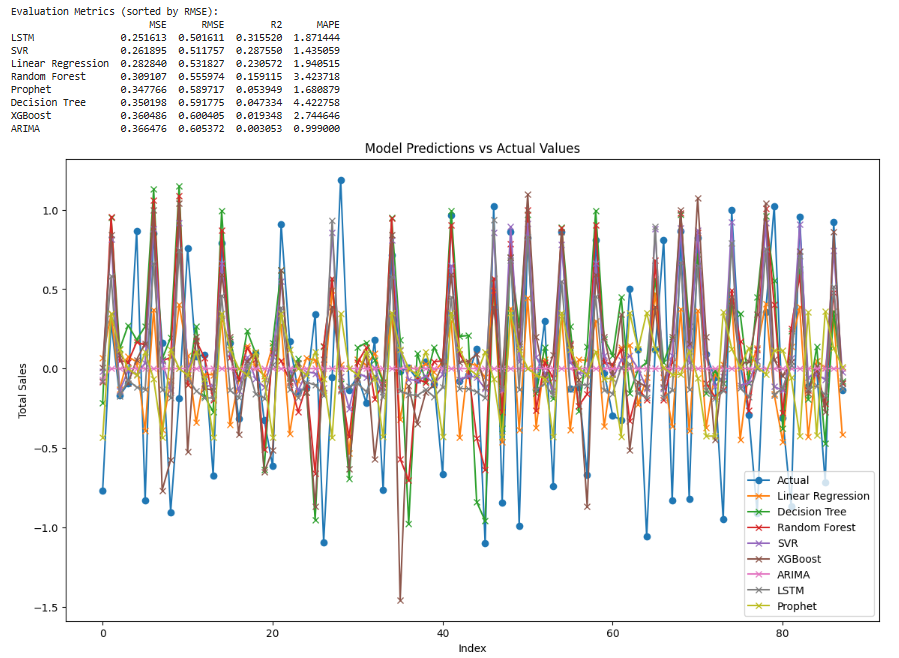
\includegraphics[width=0.9\textwidth]{2/figures/modelos_completo.png}
		\caption{Predicción Vs. valores actuales}
		\textit{Fuente: Elaboración propia}
		\label{fig11}
	\end{center}	
\end{figure}


\section{Planeamiento y descripción de actividades}
\subsection{Adquirir Base de Datos}
Este paso involucra obtener acceso a la base de datos de la empresa que contiene los registros históricos de ventas de las diferentes familias de productos. Se establecerá comunicación con los departamentos pertinentes para obtener los datos necesarios de manera segura y ética. En la Figura observamos que se adquiren las ventas desde el año 2023 al 2024, sumando más de 620 mil registros de ventas en este periodo.

\begin{figure}[H]
	\begin{center}
		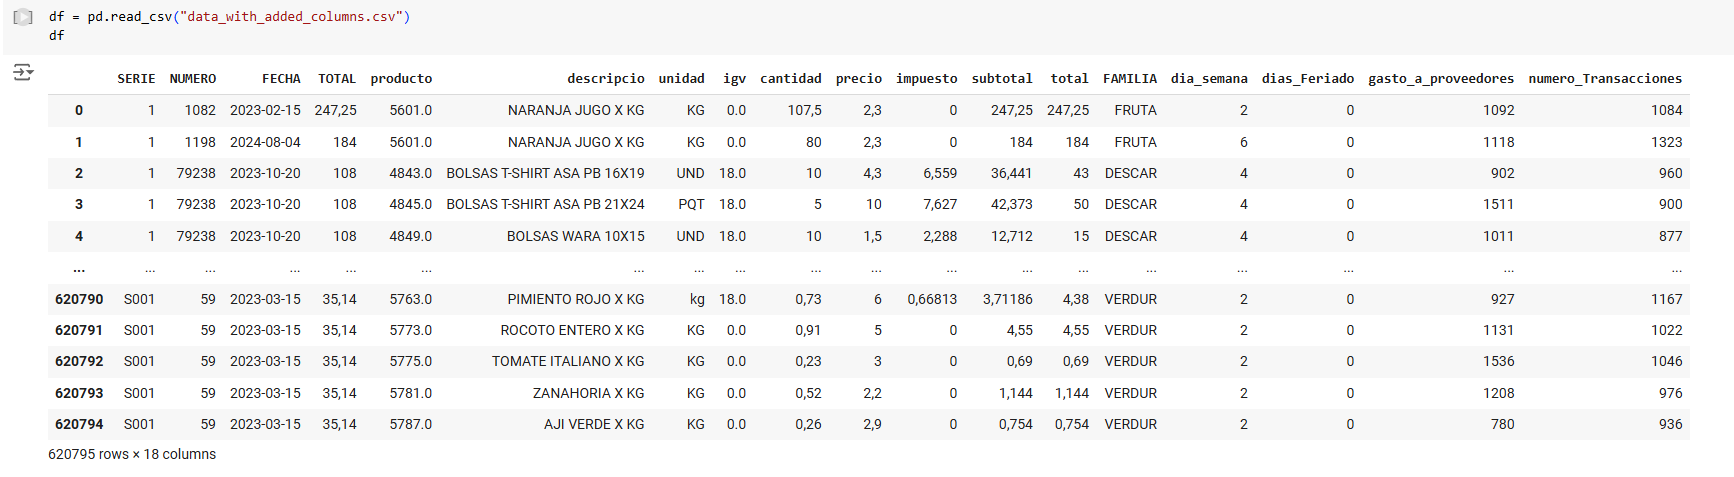
\includegraphics[width=0.9\textwidth]{2/figures/df_completa.png}
		\caption{Datos históricos de ventas}
		\textit{Fuente: Elaboración propia}
		\label{fig11}
	\end{center}	
\end{figure}

Posteriormente se decide agregar 3 nuevas columnas que serán relevantes para el pronostico de ventas. Siendo las columnas agregadas dias\_Feriado, 	gasto\_a\_proveedores y	numero\_Transacciones

\begin{figure}[H]
	\begin{center}
		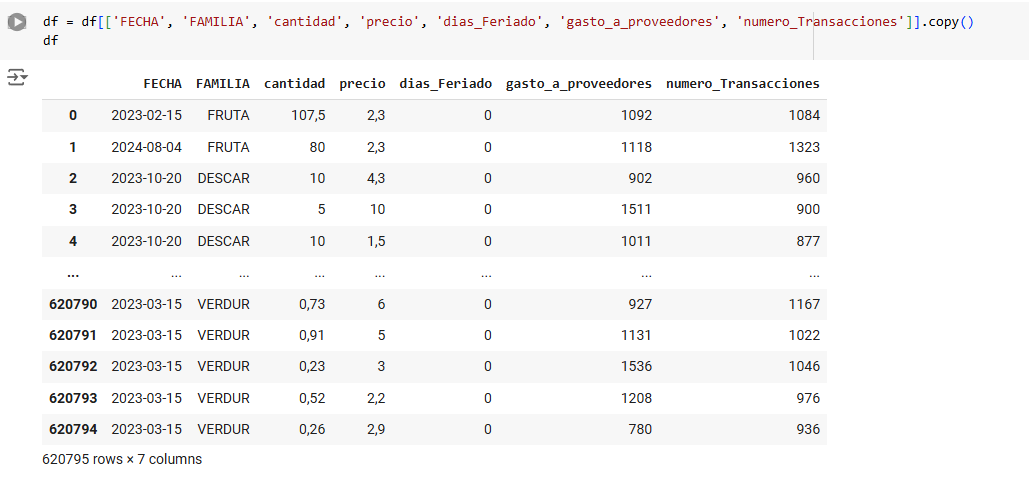
\includegraphics[width=0.9\textwidth]{2/figures/df_agregada.png}
		\caption{Datos históricos de ventas con 3 columnas agregadas}
		\textit{Fuente: Elaboración propia}
		\label{fig11}
	\end{center}	
\end{figure}


\subsection{Preprocesamiento de datos}
Antes de utilizar los datos para el análisis y modelado, es fundamental realizar un preprocesamiento adecuado. Esto incluye la limpieza de datos para eliminar valores faltantes o erróneos, la normalización para asegurar que todas las variables estén en la misma escala y la codificación de variables categóricas si es necesario. Adicional a estos pasos para asegurar la calidad, se decidio trabajar con la familia de Verduras para este analisis de Forecasting

\begin{figure}[H]
	\begin{center}
		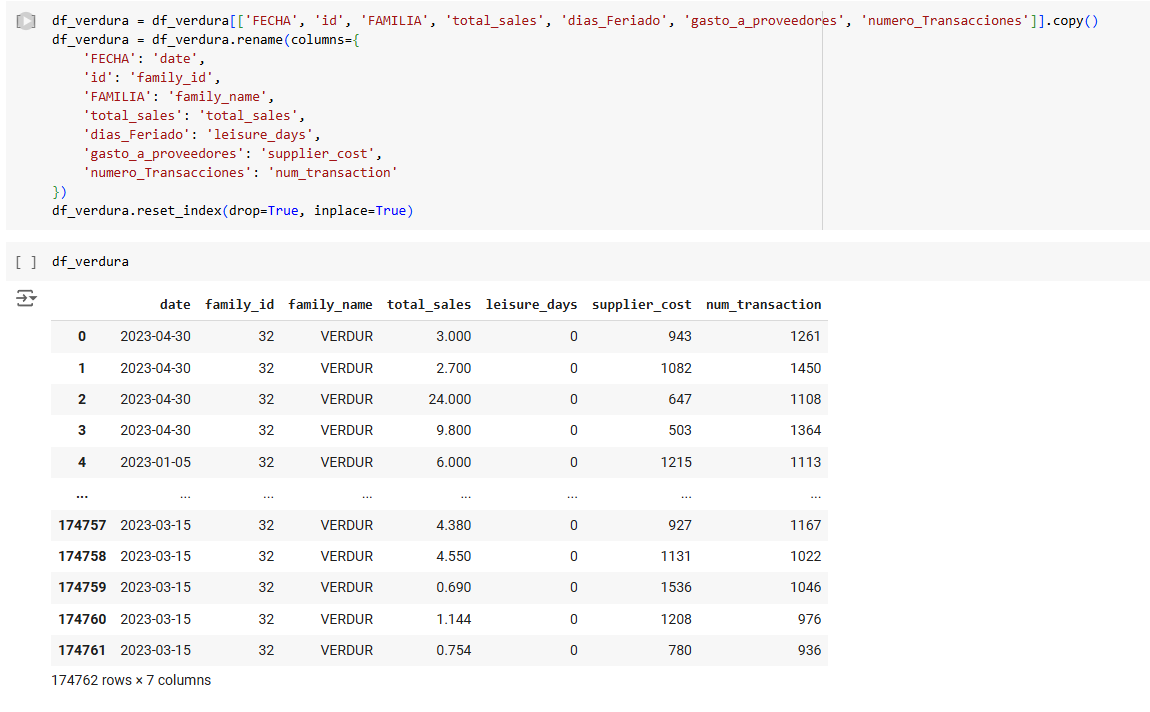
\includegraphics[width=0.9\textwidth]{2/figures/df_verduras_completa.png}
		\caption{Ventas de la familia verduras}
		\textit{Fuente: Elaboración propia}
		\label{fig11}
	\end{center}	
\end{figure}


\subsection{Selección de algoritmos a utilizar}
En este escenario, se han seleccionado los siguientes modelos para la predicción de ventas semanales de la familia de productos de verduras: Árbol de Decisión, Bosque Aleatorio, SVR, XGBoost, Regresión Lineal, ARIMA, LSTM y Prophet. Antes de proceder con el entrenamiento de estos modelos, se dividirán los datos en conjuntos de entrenamiento y prueba, asignando el 80\% de los datos para entrenamiento y el 20\% restante para pruebas.
\subsubsection{Proceso de Entrenamiento y Evaluación de Modelos}
\begin{enumerate}
	\item \textbf{División de Datos: } Los datos se dividirán en dos conjuntos:
		\begin{itemize}
			\item \textbf{Entrenamiento (80\%): } Utilizado para entrenar los modelos.
			\item \textbf{Prueba (20\%): } Utilizado para evaluar el rendimiento de los modelos.
		\end{itemize}
	\item \textbf{Entrenamiento de Modelos: } Cada uno de los modelos seleccionados se entrenará utilizando el conjunto de datos de entrenamiento. Este proceso implicará ajustar los parámetros de cada modelo para optimizar su rendimiento.
\end{enumerate}

\subsection{Definir parámetros}
Una vez seleccionados los modelos, se procederá a definir los parámetros iniciales de cada modelo y a realizar la optimización de hiperparámetros para mejorar su rendimiento predictivo. Esto se realizará utilizando técnicas como la búsqueda en cuadrícula o la optimización bayesiana. Una vez obteniendo estos parámetros se vera cual modelo es mejor para cada familia y se tomara la decisión de cual modelo trabajar con cada familia.

\begin{figure}[H]
	\begin{center}
		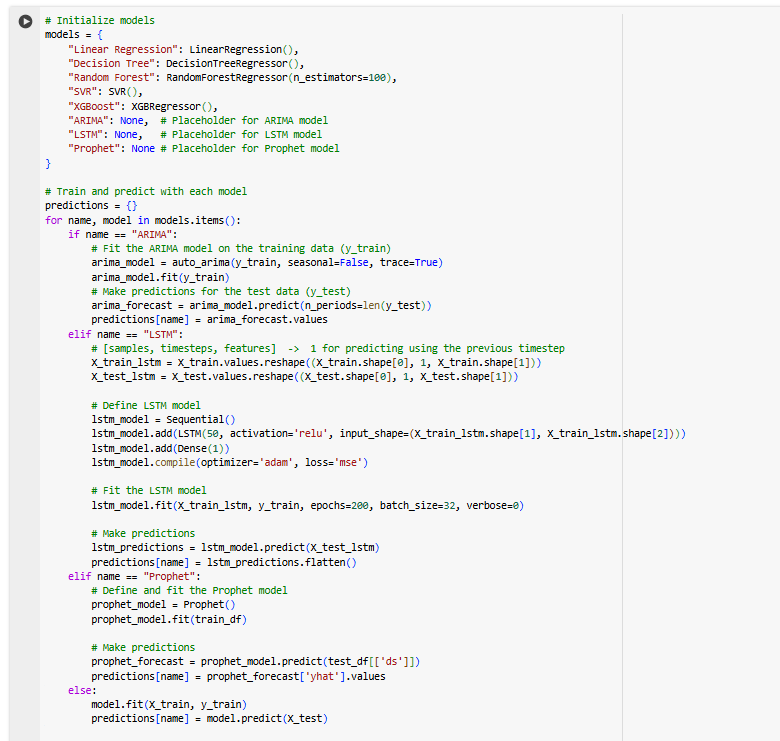
\includegraphics[width=0.9\textwidth]{2/figures/parametros_modelo.png}
		\caption{Parametros de los modelos elegidos}
		\textit{Fuente: Elaboración propia}
		\label{fig11}
	\end{center}	
\end{figure}


%
%\subsection{Obtener la predicción de cada Familia}
%Ya teniendo el modelo elegido para cada familia se comenzará a realizar la predicción para cada una de ellas y obtener las ventas futuras por semanas. Y una vez teniendo estos resultados se le brindara estos datos a los gerentes de empresa para que puedan hacerle uso a esta información.


\section{Desarrollo de actividades. Aplicación de herramientas de solución}

\subsection{Preprocesamiento de datos}
Se realizará un análisis exhaustivo para identificar y cuantificar los datos faltantes en el conjunto de datos históricos. Este análisis se llevará a cabo por columnas para determinar qué variables tienen valores ausentes y en qué medida.

%\subsection{Imputación de Datos Faltantes mediante KNN}
%Para abordar los valores faltantes identificados, se empleará el algoritmo de imputación de vecinos más cercanos (KNN). Este método permite predecir y completar los valores faltantes utilizando información de variables similares. Se seleccionará un número adecuado de vecinos para garantizar la precisión de la imputación.

%%%%%CAMBIO LISTO
\begin{figure}[H]
	\begin{center}
		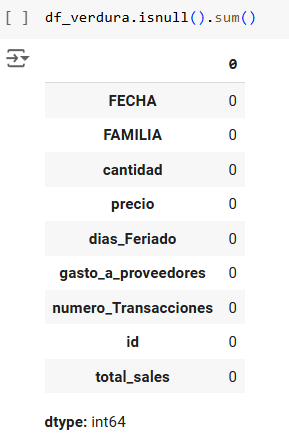
\includegraphics[width=0.4\textwidth]{2/figures/df_verdura_isnull.png}
		\caption{Identificando las columnas con datos faltantes}
		\textit{Fuente: Elaboración propia}
		\label{fig11}
	\end{center}	
\end{figure}

\subsection{Selección de Columnas relevantes}
Una vez completada la imputación de datos, se procederá a la selección de las columnas más relevantes para el análisis de predicción de ventas. En este caso, se considerarán las siguientes columnas como las más pertinentes:


%%%%%CAMBIO DE COLUMNAS LISTO
%%DATE, FAMLILY, TOTAL, LIISURE_DAYS,SUPPLIER, NUMTRANS

\begin{itemize}
	\item Date: Fecha de transacción de venta.
	\item Family\_id: Identificador unico del tipo de producto perecible
	\item Total: Medida principal de las ventas totales.
	\item Leisure\_days: Dia feriado por festividad gubernamental.
	\item Supplier\_cost: Número de pagos que se hicieron a proveedores en el día.
	\item Num\_transaction: Número de ventas en el día.
\end{itemize}
%%%CAMBIO LISSTO
\begin{figure}[H]
	\begin{center}
		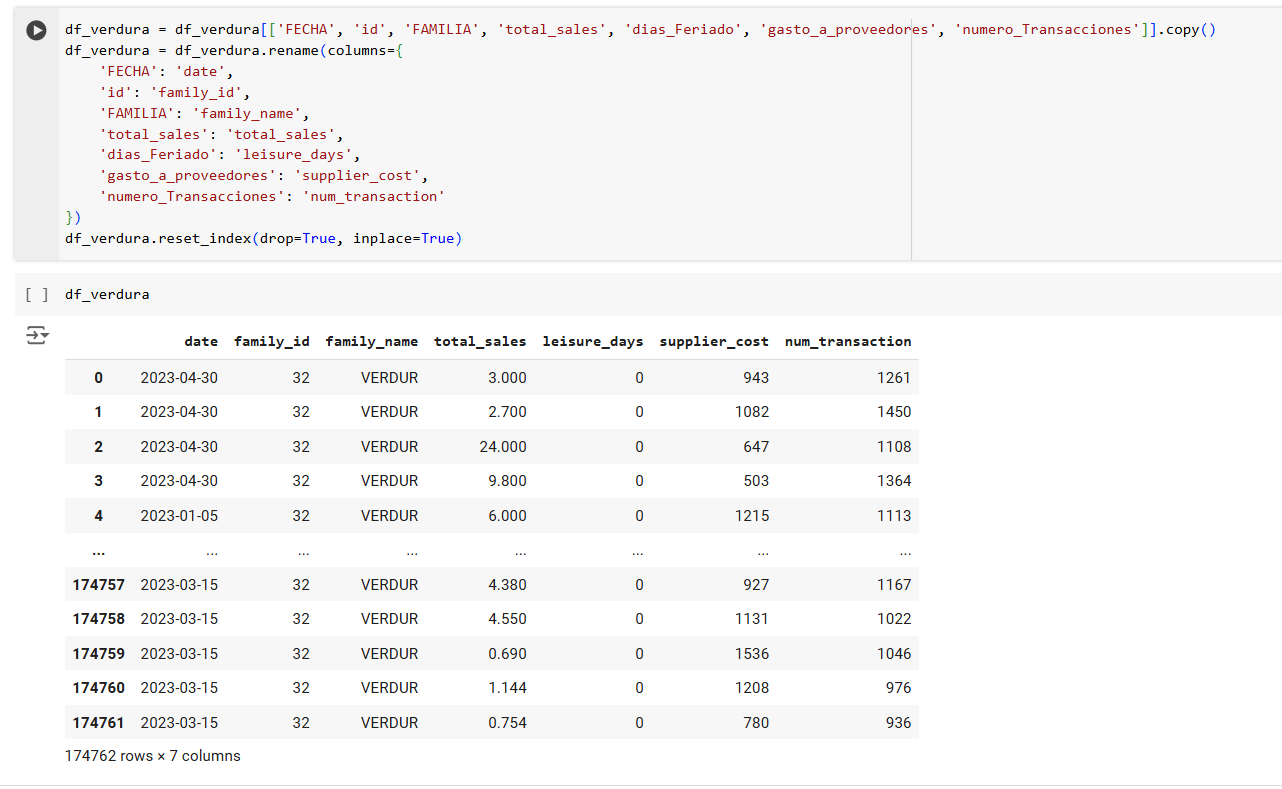
\includegraphics[width=0.7\textwidth]{2/figures/variables_dfverdura.png}
		\caption{Columnas de datos}
		\textit{Fuente: Elaboración propia}
		\label{fig11}
	\end{center}
	
\end{figure}
%%%CAMBIO LISTO
\begin{figure}[H]
	\begin{center}
		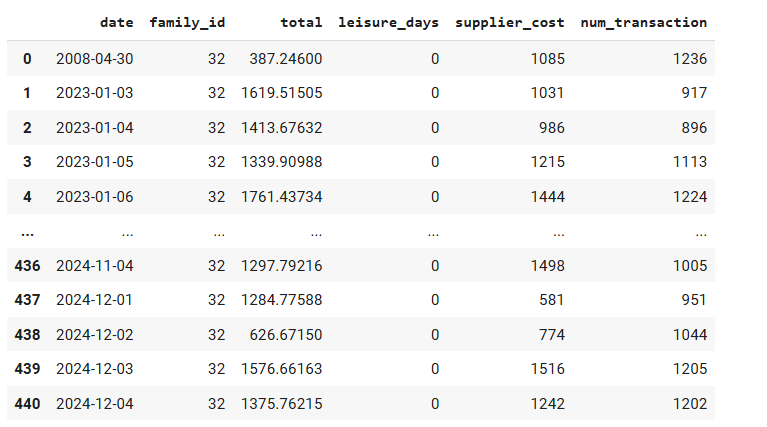
\includegraphics[width=0.7\textwidth]{2/figures/historico_ventas.png}
		\caption{Datos históricos de ventas}
		\textit{Fuente: Elaboración propia}
		\label{fig11}
	\end{center}
	
\end{figure}

\subsection{Seleccionamos los modelos a utilizar}
En este escenario, se han seleccionado los siguientes modelos: Árbol de Decisión, Random Forest, SVR, XGBoost y Regresión Lineal. Antes de proceder con el entrenamiento de estos modelos, se dividirá los datos en conjuntos de entrenamiento y prueba, asignando el 80\% de los datos para entrenamiento y el 20\% restante para pruebas.
%%CAMBIO LISTO

\begin{figure}[H]
	\begin{center}
		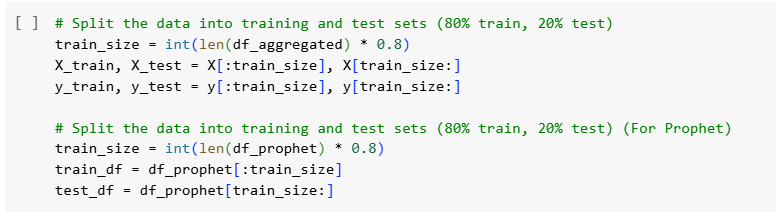
\includegraphics[width=0.7\textwidth]{2/figures/train_test.png}
		\caption{División de prueba y entrenamiento}
		\textit{Fuente: Elaboración propia}
		\label{fig11}
	\end{center}	
\end{figure}

\begin{figure}[H]
	\begin{center}
		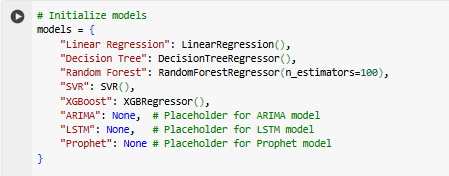
\includegraphics[width=0.7\textwidth]{2/figures/modelos.png}
		\caption{Modelos elegidos}
		\textit{Fuente: Elaboración propia}
		\label{fig11}
	\end{center}	
\end{figure}


A continuación se vera como se entrenan los modelos y las métricas que se eligieron que vendrían a ser RMSE, MSE, R2 y MAPE
%LISTO
\begin{figure}[H]
	\begin{center}
		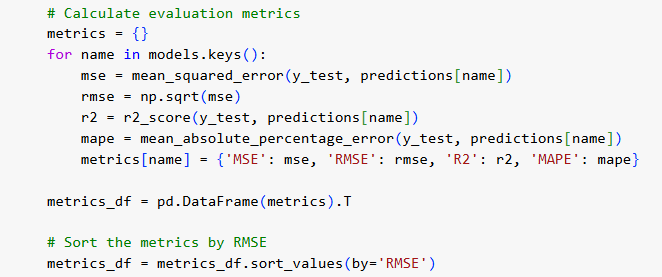
\includegraphics[width=0.7\textwidth]{2/figures/metricas_df.png}
		\caption{Definicion de modelos  y métricas}
		\textit{Fuente: Elaboración propia}
		\label{fig11}
	\end{center}
	
\end{figure}

%\begin{figure}[H]
%	\begin{center}
%		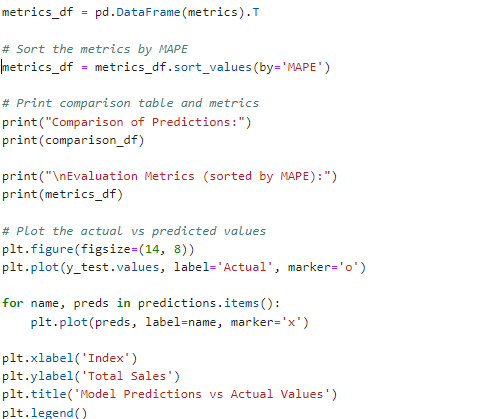
\includegraphics[width=0.7\textwidth]{2/figures/mape2.png}
%		\caption{}
%		\label{fig11}
%	\end{center}
%	
%\end{figure}

A continuación se vera la comparación de todos los modelos y apartir de eso se eligira el mejor modelo para trabajar con una familia.


\begin{figure}[H]
	\begin{center}
		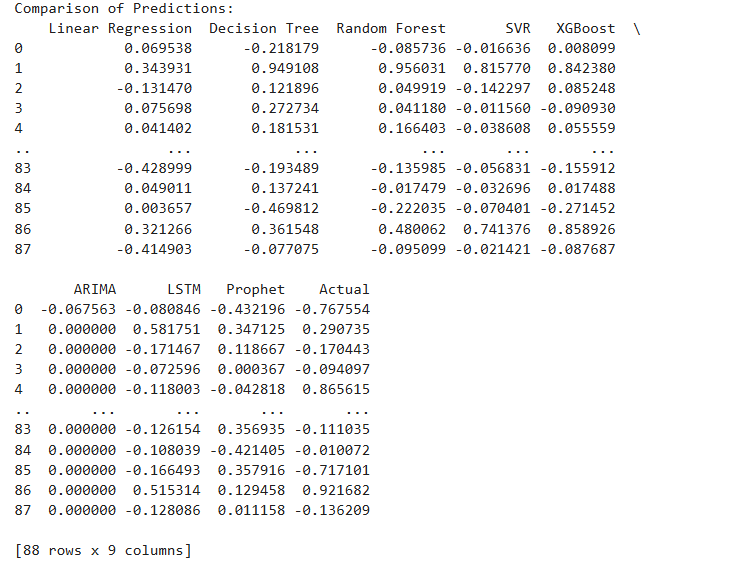
\includegraphics[width=0.8\textwidth]{2/figures/comparacion_modelos.png}
		\caption{Comparación de resultados}
		\label{fig22}
	\end{center}
	
\end{figure}


\begin{figure}[H]
	\begin{center}
		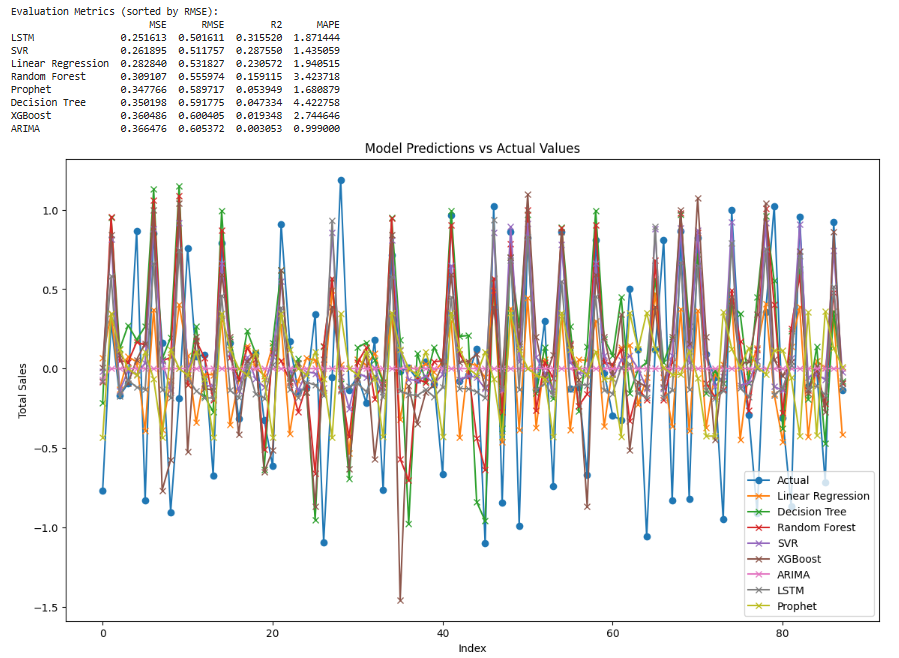
\includegraphics[width=0.8\textwidth]{2/figures/modelos_completo.png}
		\caption{Resultados de modelos}
		\label{fig23}
	\end{center}
	
\end{figure}
%
%\begin{figure}[H]
%	\begin{center}
%		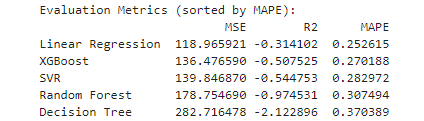
\includegraphics[width=0.7\textwidth]{2/figures/metricas.png}
%		\caption{}
%		\label{fig231}
%	\end{center}
%	
%\end{figure}



\section{Medición de la solución}
%%%%AGREGAR RMSE R2 LISTO
Los parámetros que se utilizaron para poder elegir el mejor modelo son los siguientes:

Raíz del error cuadrático medio (RMSE): El término utilizado para denotar el error que surge de la diferencia entre los valores predichos y los valores observados por un modelo o estimador es conocido como error cuadrático medio (RMSE). Esta medida se obtiene al calcular la raíz cuadrada de la media de los errores cuadráticos, lo cual refleja la disparidad entre los valores reales y los valores pronosticados. Es importante destacar que el RMSE, al ser siempre positivo, donde valores menores indican un ajuste más acertado de los datos al modelo. La formulación de este concepto se detalla en la siguiente sección.

\begin{equation}  
	\label{eq:RMSE}
	\hat{y}_i = \sqrt{\frac{\sum_{i=1}^{n} (y_i - \hat{y}_i)^2}{n}}
\end{equation}


Error Cuadrático Medio (MSE - Mean Squared Error): El MSE mide el promedio de los cuadrados de los errores entre las ventas reales y las ventas predichas por el modelo de regresión lineal. En otras palabras, indica cuán cerca están las ventas predichas de las ventas reales en términos de la diferencia cuadrada entre ellos.

\begin{equation}  
	\label{eq:MSE}
	\hat{\text{MSE} = \frac{1}{n} \sum_{i=1}^{n} (y_i - \hat{y}_i)^2
	}
\end{equation}

Error Porcentual Absoluto Medio (MAPE - Mean Absolute Percentage Error): El MAPE proporciona una medida de la precisión relativa del modelo de regresión lineal en términos porcentuales. Mide el promedio de los errores porcentuales absolutos entre las ventas reales y las ventas predichas. Esto te permite comprender cuánto se desvían, en promedio, las ventas predichas de las ventas reales en términos de porcentaje.

\begin{equation}  
	\label{eq:MAPE}
	\hat{\text{MAPE} = \frac{1}{n} \sum_{i=1}^{n} \left| \frac{y_i - \hat{y}_i}{y_i} \right| \times 100\%
	}
\end{equation}

Coeficiente de determinación: El valor del coeficiente de determinación (R2) oscila entre 0 y 1, reflejando la fracción de puntos en un conjunto de datos que se ajustan a la línea de regresión. Este coeficiente es una medida de la cantidad de variabilidad de la variable dependiente que puede ser explicada por el modelo de regresión. En el contexto de modelos estadísticos, R2 se emplea para predecir resultados futuros o validar hipótesis, siendo una herramienta crucial para evaluar la calidad del modelo y la proporción de variación en los resultados que este puede explicar. La formulación de R2 se presenta en la siguiente línea. (Bruce, P. et al. 2020)

\begin{equation}  
	\label{eq:r2}
	\hat{R}^2 = 1 - \frac{\sum_{i=1}^{n} (y_i - \hat{y}_i)^2}{\sum_{i=1}^{n}(y_i- \bar{y})^2}
\end{equation}



\subsection{Simulación de la predicción}
Se realizo la simulación a la familia que tiene más relevancia ósea “VERDURAS” como se menciono en el anterior punto se utilizo el modelo de regresión lineal ya que mostro mejores resultados en los parámetros RMSE, MSE ,R2 y MAPE. A continuación muestro el código con el que se trabajo para realizar la simulación de la predicción

%%CAMBIO 
\begin{figure}[H]
	\begin{center}
		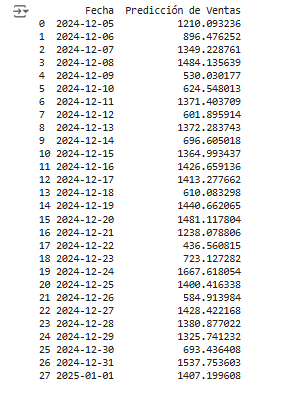
\includegraphics[width=0.5\textwidth]{2/figures/resultadofinal_numerico.png}
		\caption{Predicción numerica del mejor modelo}
		\textit{Fuente: Elaboración propia}
		\label{fig231}
	\end{center}	
\end{figure}


\begin{figure}[H]
	\begin{center}
		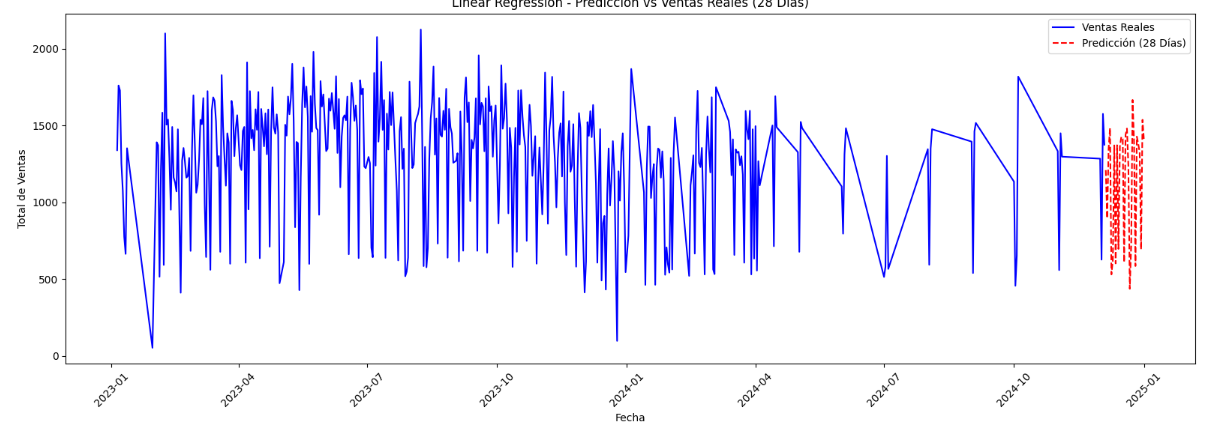
\includegraphics[width=0.9\textwidth]{2/figures/resultadofinal.png}
		\caption{Predicción con el mejor modelo}
		\textit{Fuente: Elaboración propia}
		\label{fig231}
	\end{center}	
\end{figure}



%En este código se utiliza Matplotlib para crear un gráfico que representa la predicción de ventas totales. Primero, se establece el tamaño de la figura. Luego, se trazan los datos de entrenamiento y prueba, así como las predicciones del mejor modelo. Se añade una línea vertical para indicar la división entre los conjuntos de entrenamiento y prueba. Y como resultado se obtiene:
%%%CAMBIO
%\begin{figure}[H]
%	\begin{center}
%		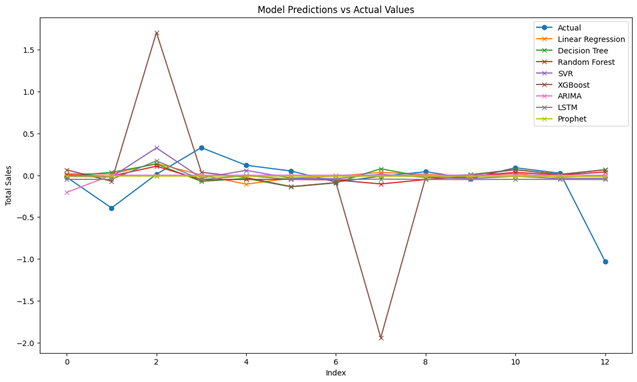
\includegraphics[width=0.9\textwidth]{2/figures/predict_Vs_actual.png}
%		\caption{Predicción Vs. valores actuales}
%		\textit{Fuente: Elaboración propia}
%		\label{fig11}
%	\end{center}	
%\end{figure}